\section{Auswertung}
\label{sec:Auswertung}
Die Umskalierung von Messwinkel auf die entsprechende Energie erfolgte über die Bragg-Bedingung $E = \frac{hc}{2d\sin(\theta)}$ via Python \cite{matplotlib} \cite{numpy} \cite{uncertainties}.

\subsection{Bragg-Bedingung}
\label{sec:bragg}

Der Erwartungswert für das Intensitätsmaximum liegt bei $\gamma = 2*theta = 28\si{\degree} $, in diesem Versuch wurde es jedoch bei $26\si{\degree}$ gemessen, wie sich Abb. \ref{fig:bragg} entnehmen lässt.

\begin{figure}
  \centering
  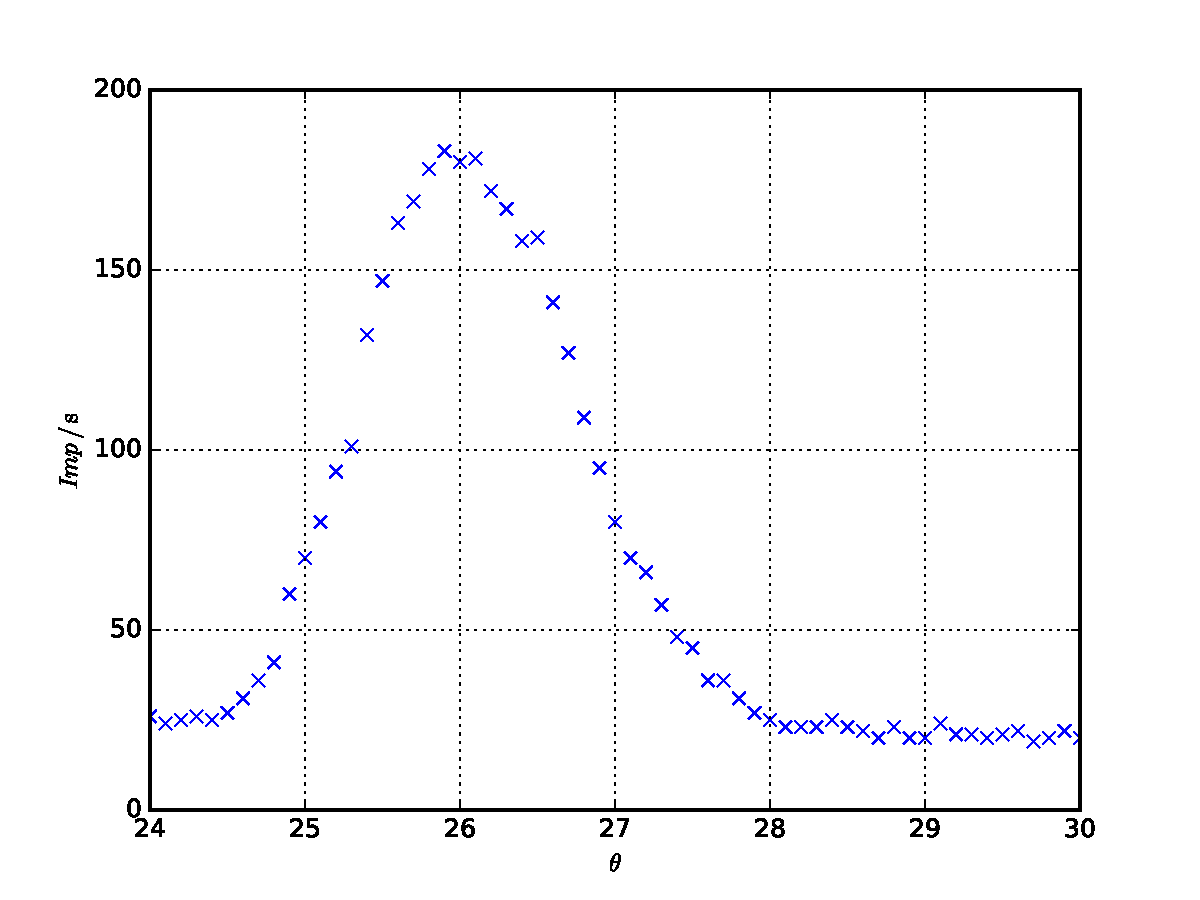
\includegraphics[width=\textwidth]{./Python/bragg.pdf}
  \caption{Zählrate aufgetragen gegen den Winkel $\gamma$ (in Grad) zwischen Röntgenstrahl und Zählrohr bei einem Kristallwinkel von $\theta = 14 \si{\degree}$.}
  \label{fig:bragg}
\end{figure}

\subsection{Emissionsspektrum}
\label{sec:emission}

\begin{figure}
  \centering
  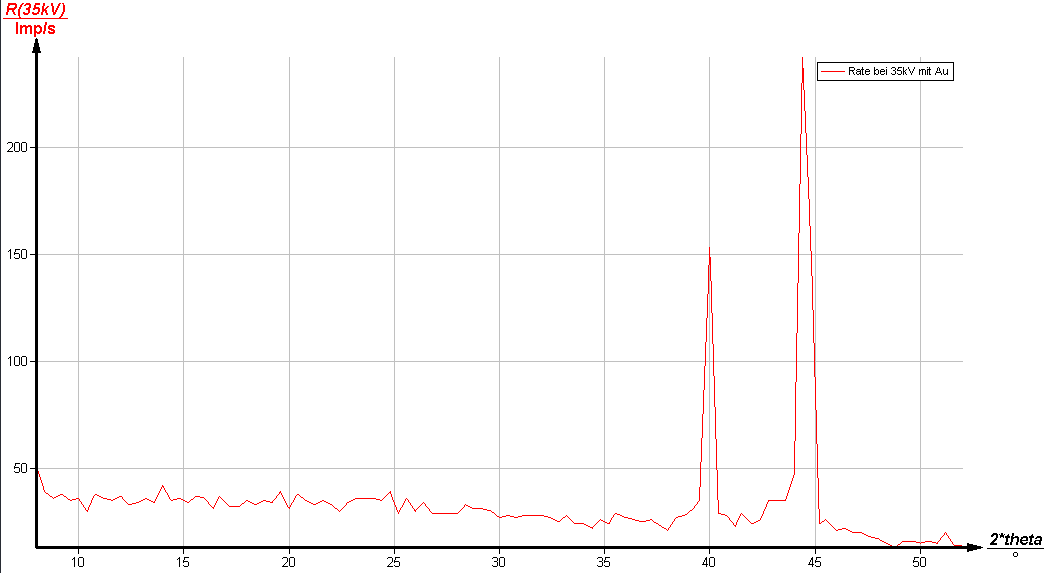
\includegraphics[height = 7cm]{./Messdaten/Cu.PNG}
  \caption{Gemessenes Röntgenspektrum der verwendeten Kupferröhre}
  \label{fig:brems}
\end{figure}

Die maximale Energie der in der Apparatur auftretenden Röntgenquanten beträgt durch die verwendete Beschleunigungsspannung bedingt $\SI{35}{\kilo \eV}$. Es sollte somit im in Abb. \ref{fig:brems} dargestellten Spektrum ein Bremsberg erkennbar sein, mit einer maximalen Energie von $\SI{35}{\kilo \eV}$. Diese Grenze lässt sich jedoch nicht nachweisen.

\begin{figure}
  \centering
  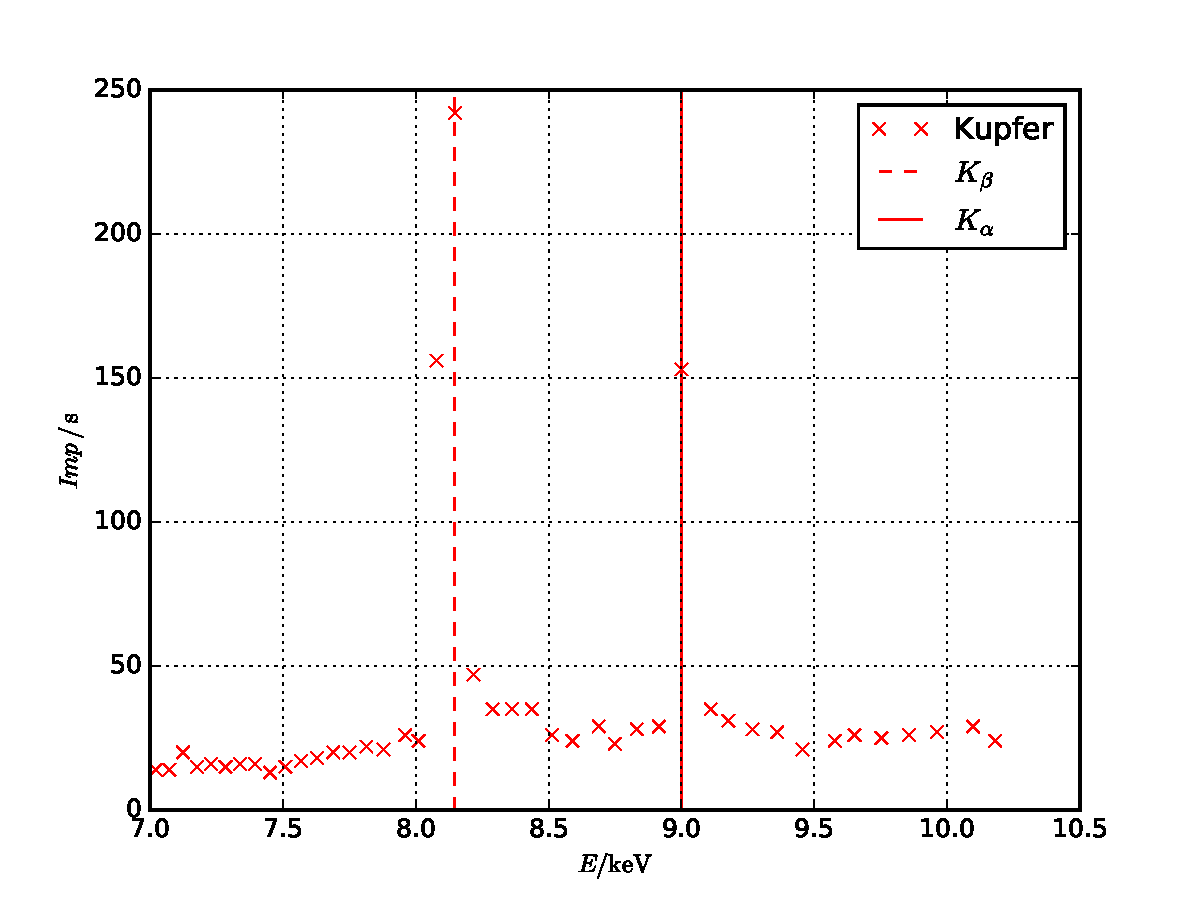
\includegraphics[height = 7cm]{./Python/Kupfer.pdf}
  \caption{Spektrum der verwendeten Kupfer-Röntgenröhre, eingeschränkt auf $\SI{7}{\kilo \eV}$ bis $\SI{10.5}{\kilo \eV}$.
  \label{fig:klinie}
\end{figure}

Aus Abb. \ref{fig:klinie} lassen sich die Werte $K_\beta = \SI{9}{\kilo \eV}$ und $K_\alpha = \SI{8.15}{\kilo \eV}$ der klar erkennbaren $K_\alpha$- bzw. $K_\beta$-Linie entnehmen. Die Halbwertsbreite der $K_\alpha$-Linie beträgt $\Delta E_\alpha = 0.05 \,\si{\kilo \eV}$, die der $K_\beta$-Linie $\Delta E_\beta = 0.09 \, \si{\kilo \eV}$. Die Auflösung entspricht dann etwa $0.1-0.2 \si{\kilo \eV}$, da sich zwei Peaks, deren Halbwertsbreiten nicht überlappen zweifelsfrei unterscheiden lassen.


\subsection{Absorbtionsspektrum}
\label{sec:absorption}
Aus Abb. \ref{fig:brom} lassen sich für die K-Kanten der verwendeten Elemente die in Tabelle \ref{tab:Kkanten} dargestellten Werte entnehmen. Zusätzlich wurden die Abschirmungskonstanten $\sigma_K$ aus Formel \eqref{eqn:be} berechnet.

\begin{table}
  \centering
  \caption{Aus der Messung des Beugungsspektrums gewonnene K-Kanten-Energien und Abschirmungskonstanten, mit Abweichungen zur Theorie. \cite{princeton}.}
  \label{tab:Kkanten}
  \begin{tabular}{|c|c|c|c|c|c|c|}
    \toprule
    Element & $E_K$/keV & $E_{theo}$/keV & $\Delta E$ /keV & $\sigma_K$ & $\sigma_{theo}$ & $\Delta \sigma$ \\
    \midrule
    Zn & 9.5 & 9.65 & 0.2 & 3.57 & 3.36 & 0.21\\
    Ge & 11.0 & 11.1 & 0.1 & 3.56 & 3.42 & 0.13\\
    Br  & 13.5 & 13.47 & 0.1 & 3.49 & 3.53 & 0.04\\
    Sr  & 16.0 & 16.1 & 0.1 & 3.70 & 3.59 & 0.11\\
    Zr  & 18.0 & 18.0 & 0.0 & 3.62 & 3.62 & 0.0 \\
    \bottomrule
    \end{tabular}
\end{table}

Mit diesen Werten lässt sich durch den in Abb. \ref{fig:moseley} dargestellten linearen Fit ($f=E_{ryd} Z^2 +b$) über das Moseley-Gesetz ($E = E_{ryd} Z_eff^2$) die Rydbergenergie zu
\begin{equation*}
  E_{ryd} = \SI{12.08 \pm 0.11}{\eV}
\end{equation*}
bestimmen ($b= \SI{-1.36 \pm 0.14}{\kilo \eV}$).

\begin{figure}
  \centering
  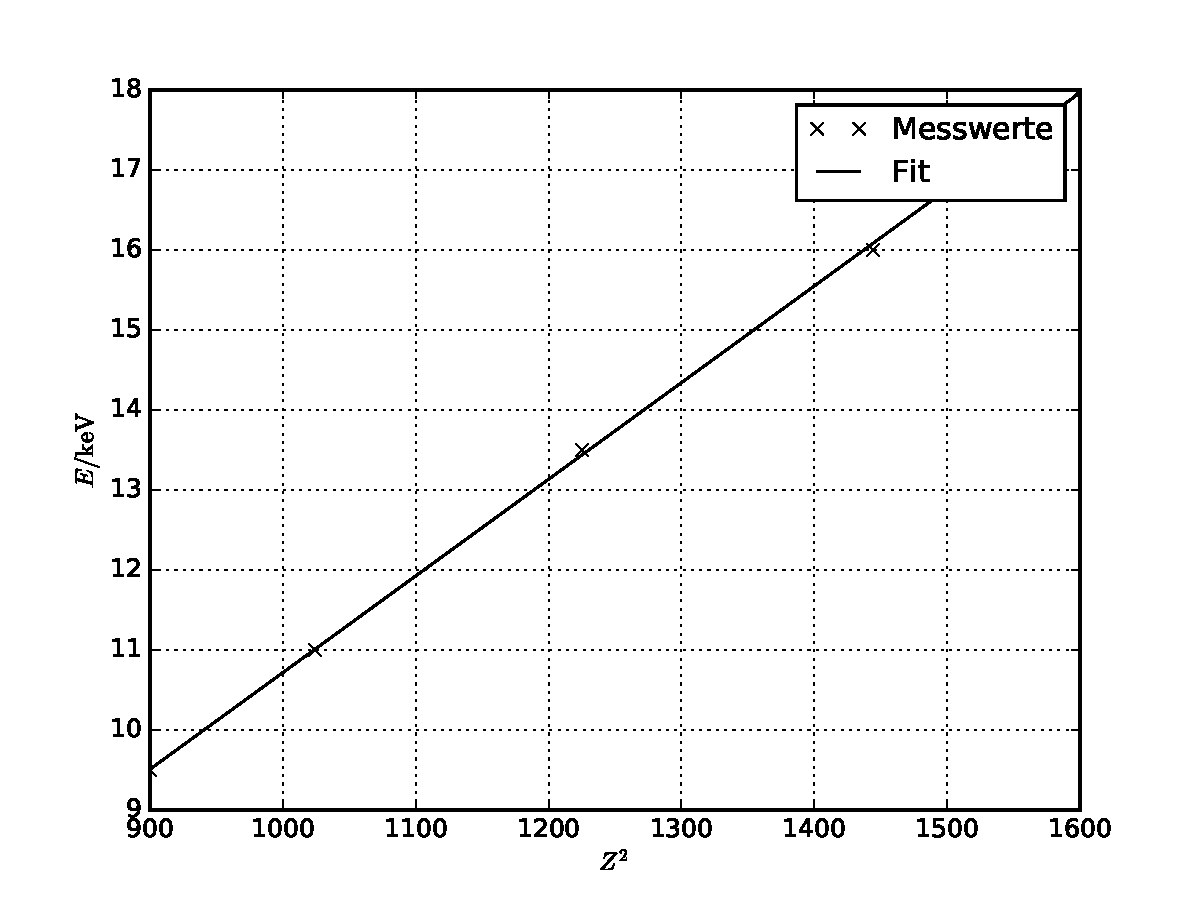
\includegraphics[height = 7cm]{./Python/Mosley.pdf}
  \caption{Bestimmung der Rydbergenergie durch linearen Ausgleich}
  \label{fig:moseley}
\end{figure}

\begin{figure}
  \centering
  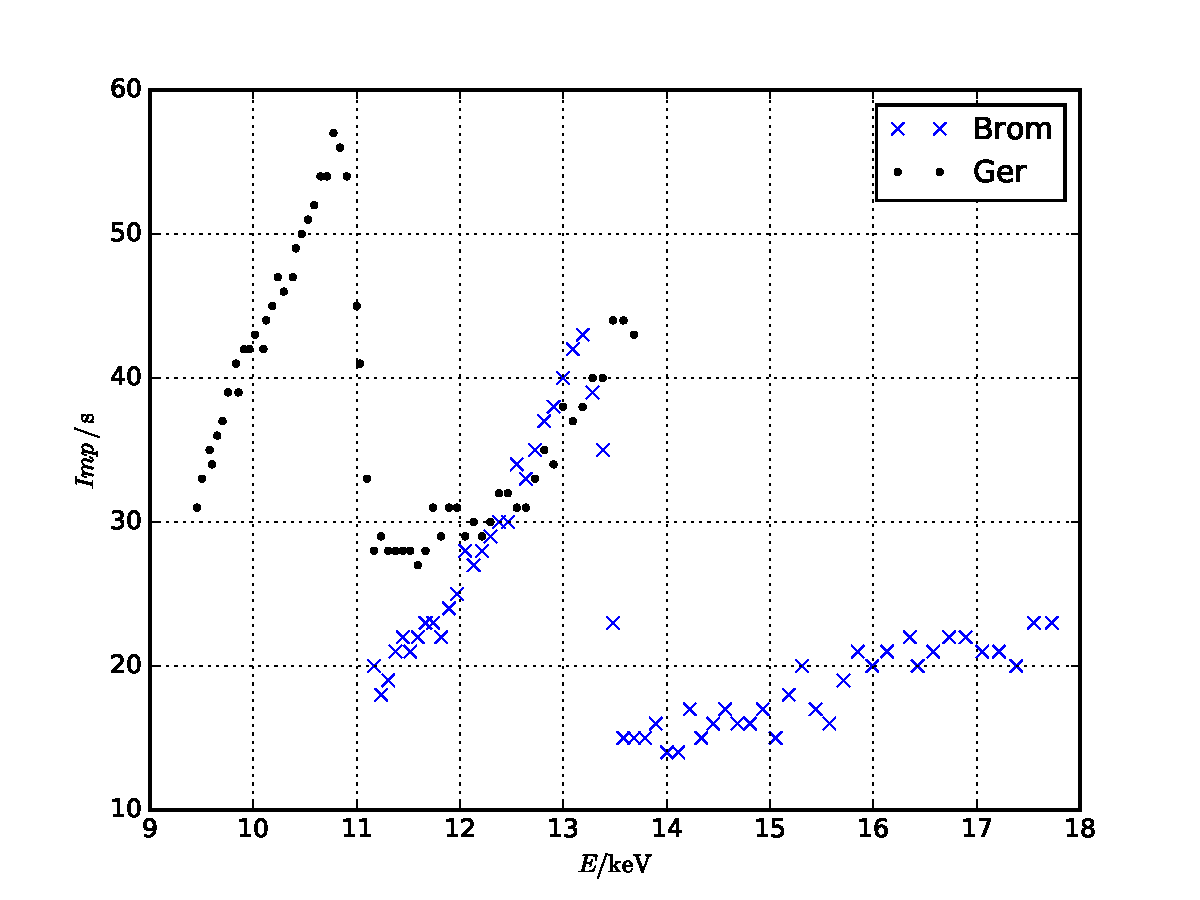
\includegraphics[height = 7cm]{./Python/Brom.pdf}
  \caption{Messung der vom Kristall gebeugten Röntgenstrahlung unter Verwendung eines Brom-Absorbers.}
  \label{fig:brom}
\end{figure}


\begin{figure}
  \centering
  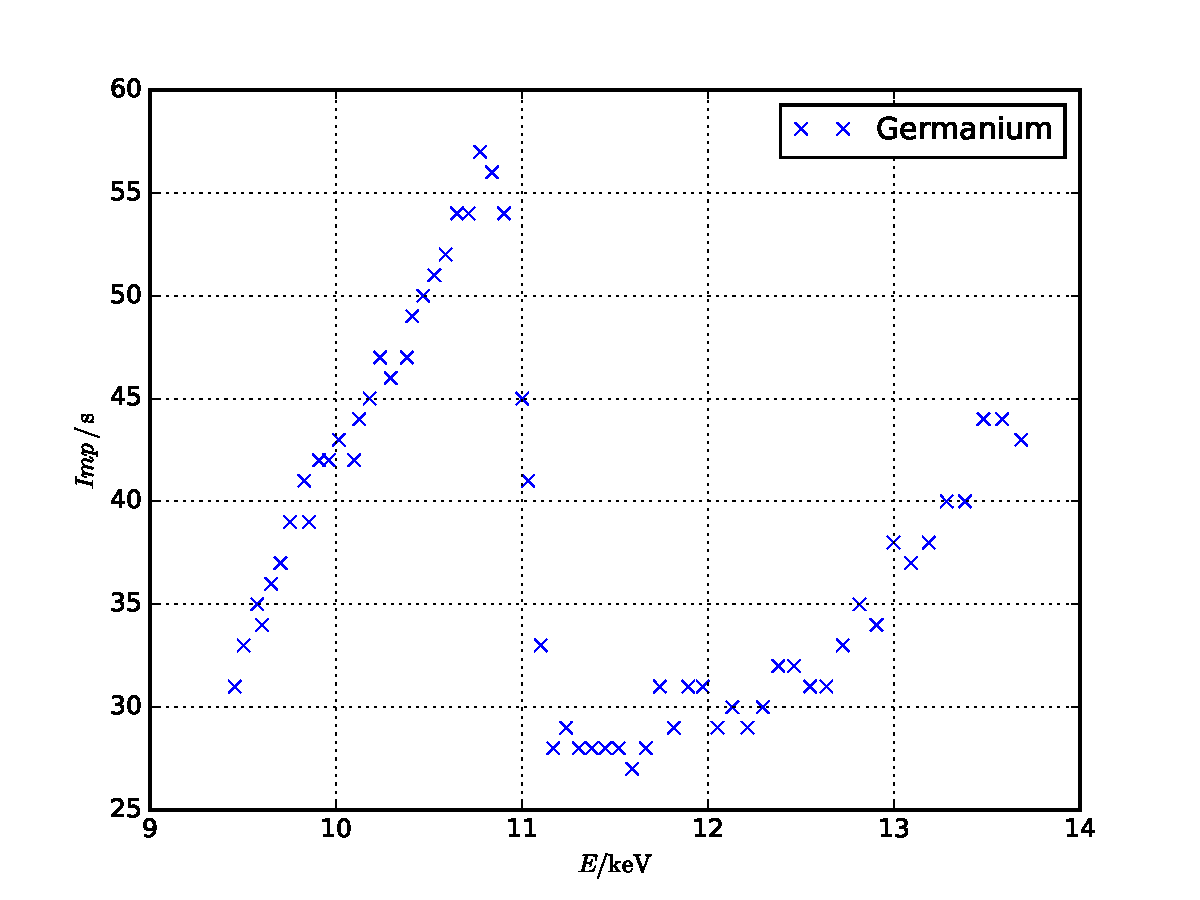
\includegraphics[height = 7cm]{./Python/Ger.pdf}
  \caption{Messung der vom Kristall gebeugten Röntgenstrahlung unter Verwendung eines Germanium-Absorbers.}
  \label{fig:ger}
\end{figure}


\begin{figure}
  \centering
  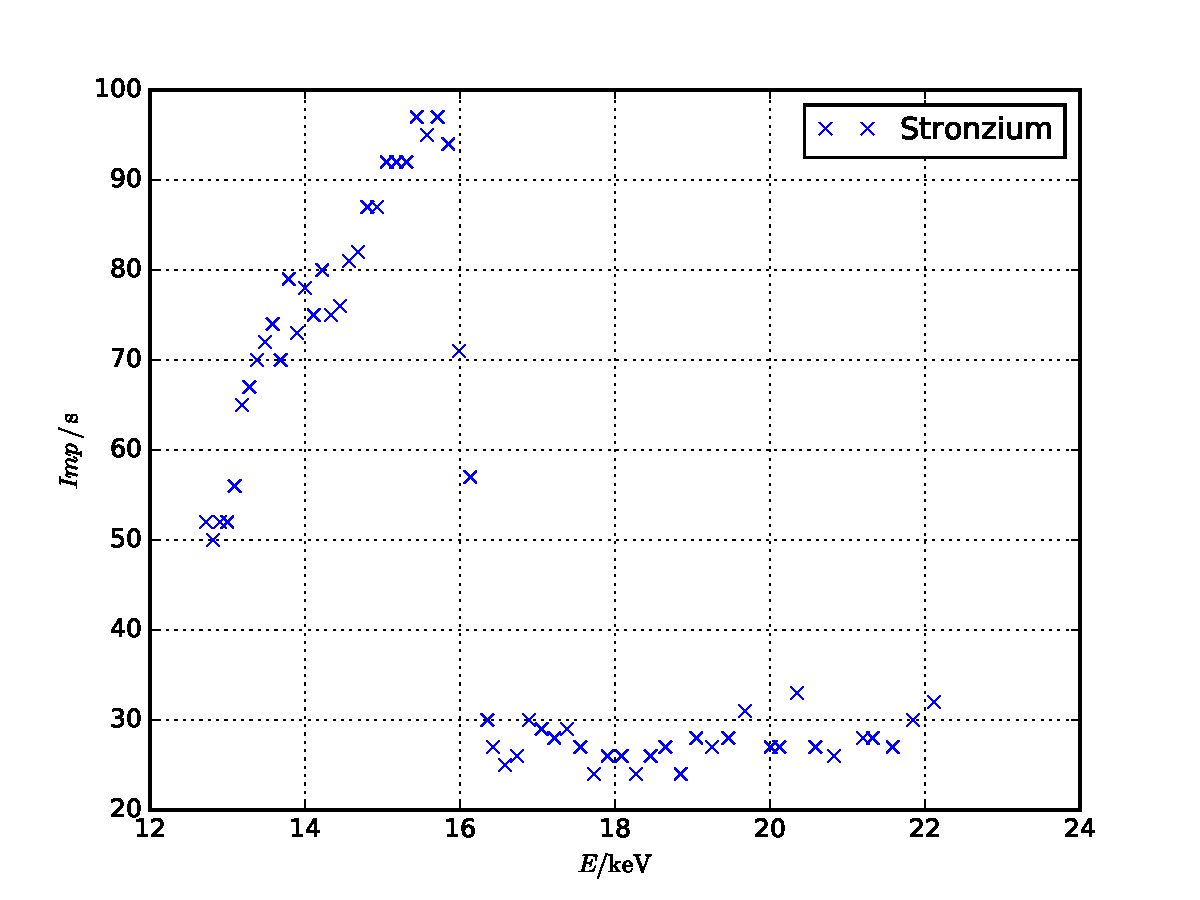
\includegraphics[height = 7cm]{./Python/stronz.pdf}
  \caption{Messung der vom Kristall gebeugten Röntgenstrahlung unter Verwendung eines Stronzium-Absorbers.}
  \label{fig:stronz}
\end{figure}



\begin{figure}
  \centering
  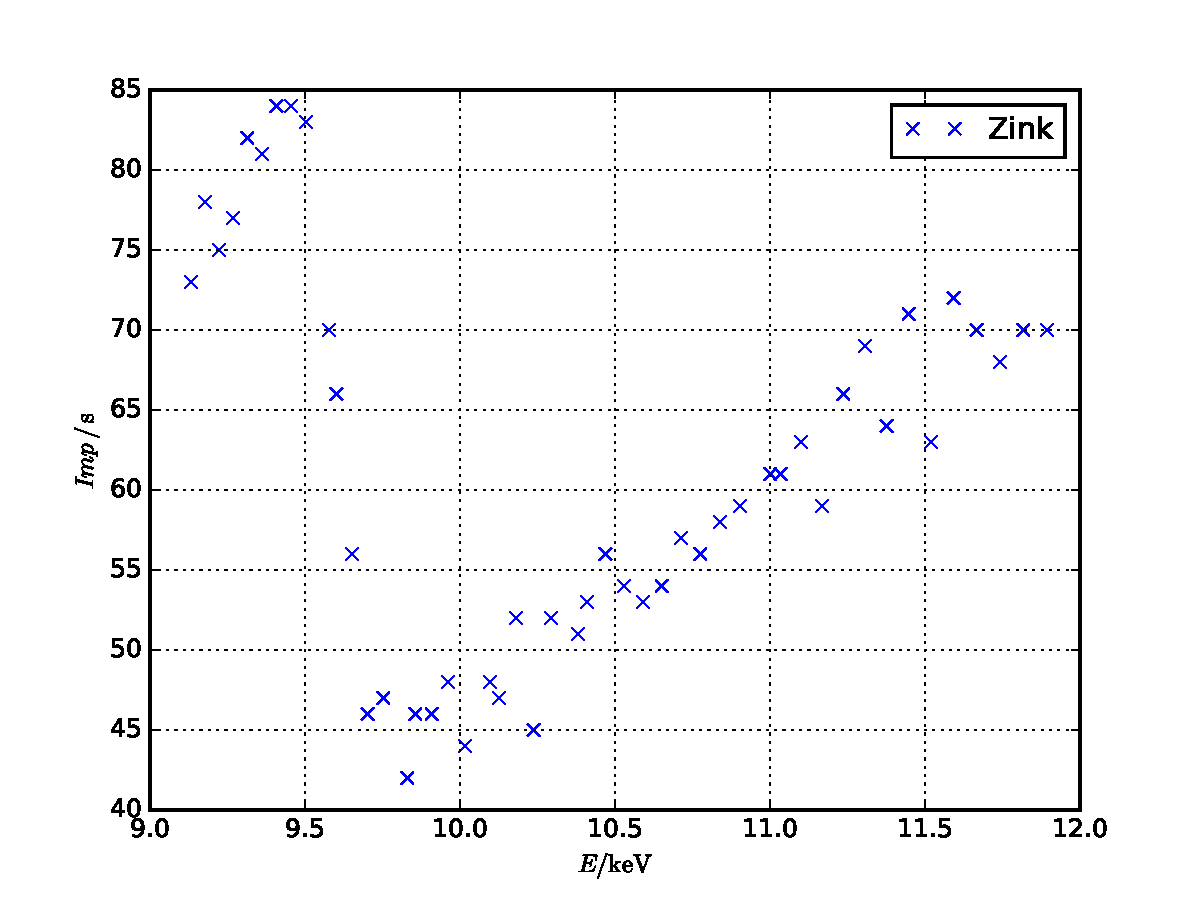
\includegraphics[height = 7cm]{./Python/zink.pdf}
  \caption{Messung der vom Kristall gebeugten Röntgenstrahlung unter Verwendung eines Zink-Absorbers.}
  \label{fig:zink}
\end{figure}



\begin{figure}
  \centering
  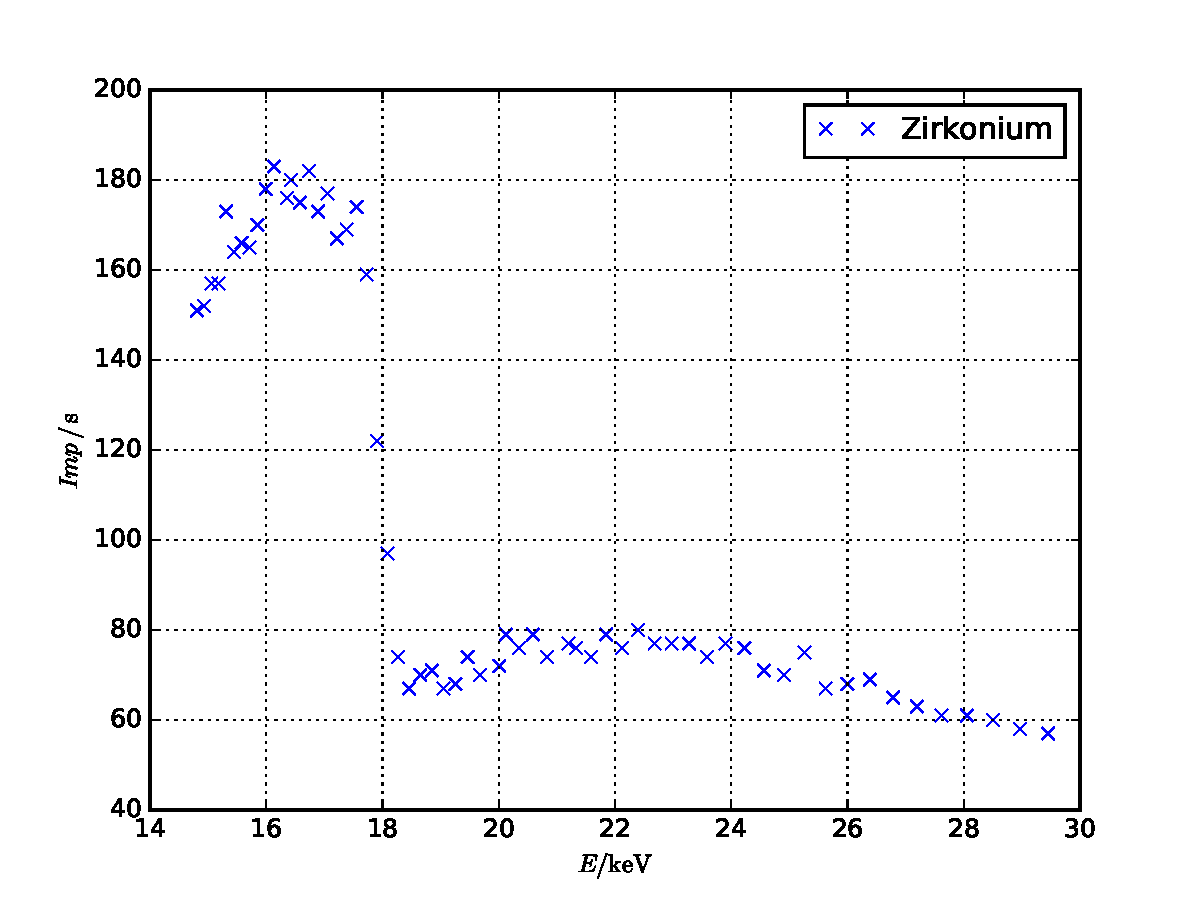
\includegraphics[height = 7cm]{./Python/zirk.pdf}
  \caption{Messung der vom Kristall gebeugten Röntgenstrahlung unter Verwendung eines Zirkonium-Absorbers.}
  \label{fig:brom}
\end{figure}

Für Quecksilber liegt der Erwartungswert der $L_2$-Kante bei 14.2keV, für die $L_3$-Kante bei 12.3keV \cite{skuld}. Die aus Abb. \ref{fig:queck} abgelesenen Werte betragen $E_{L2} = 13.8 \si{\kilo \eV}$ und $E_{L3} = 12$keV ($\Delta E_2 = 0.4$keV, $\Delta E_3 = 0.3$keV).
Hierraus lässt sich $\sigma_L$ über die Formel

\begin{equation}
  \sigma_L = Z - \left(\frac{4}{\alpha}\sqrt{\frac{\Delta E_L}{E_{ryd}}}-\frac{5\Delta E_L}{E_{ryd}}\right)^{\frac{1}{2}} \left(1+\alpha^2   \frac{19\Delta E_L}{32 E_{ryd}}\right)^{\frac{1}{2}}
\end{equation}

mit $\alpha = 7.3 \cdot 10^{-3}$ als der Sommerfeldschen Strukturkonstante und den Literaturwerten $E_K = 83.1$keV \cite{skuld} und $\sigma_K = 1.8$ berrechnen zu $\sigma_L = 4.89$.

\begin{figure}
  \centering
  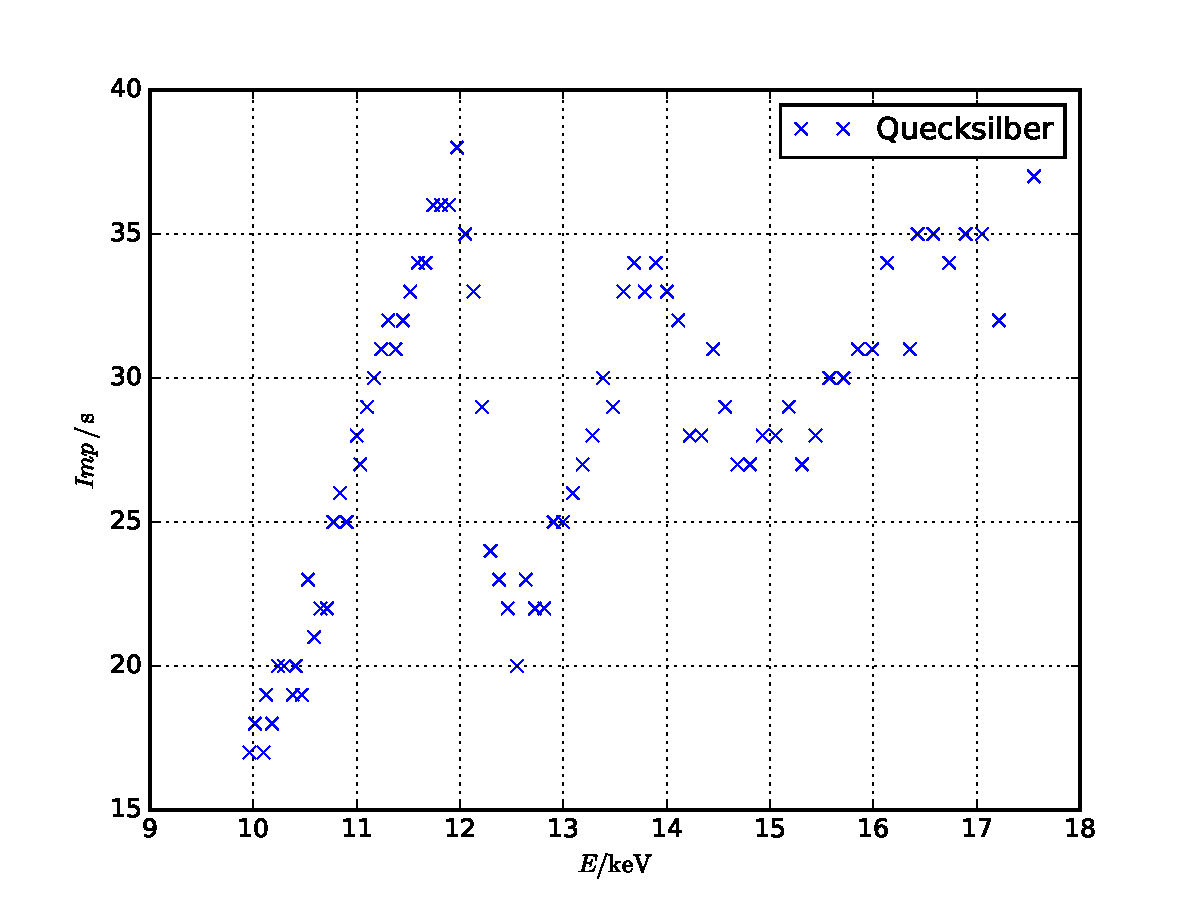
\includegraphics[height = 5cm]{./Python/queck.pdf}
  \caption{Messung der vom Kristall gebeugten Röntgenstrahlung unter Verwendung eines Quecksilber-Absorbers.}
  \label{fig:queck}
\end{figure}
